\documentclass[../main.tex]{subfiles}
\graphicspath{{\subfix{../images/}}}
\begin{document}

\chapter{RESULTADOS}

\section{Experimentos y Resultados}

\trainplot{Primer entrenamiento (Synthdog)}{train_es_synthdog.csv}{train_es_synthdog_val.csv}
\trainplot{Segundo entrenamiento (Documentos sintéticos)}{train_es_finetuned_docvqa.csv}{train_es_finetuned_docvqa_val.csv}

\begin{figure}[H]
	\centering
	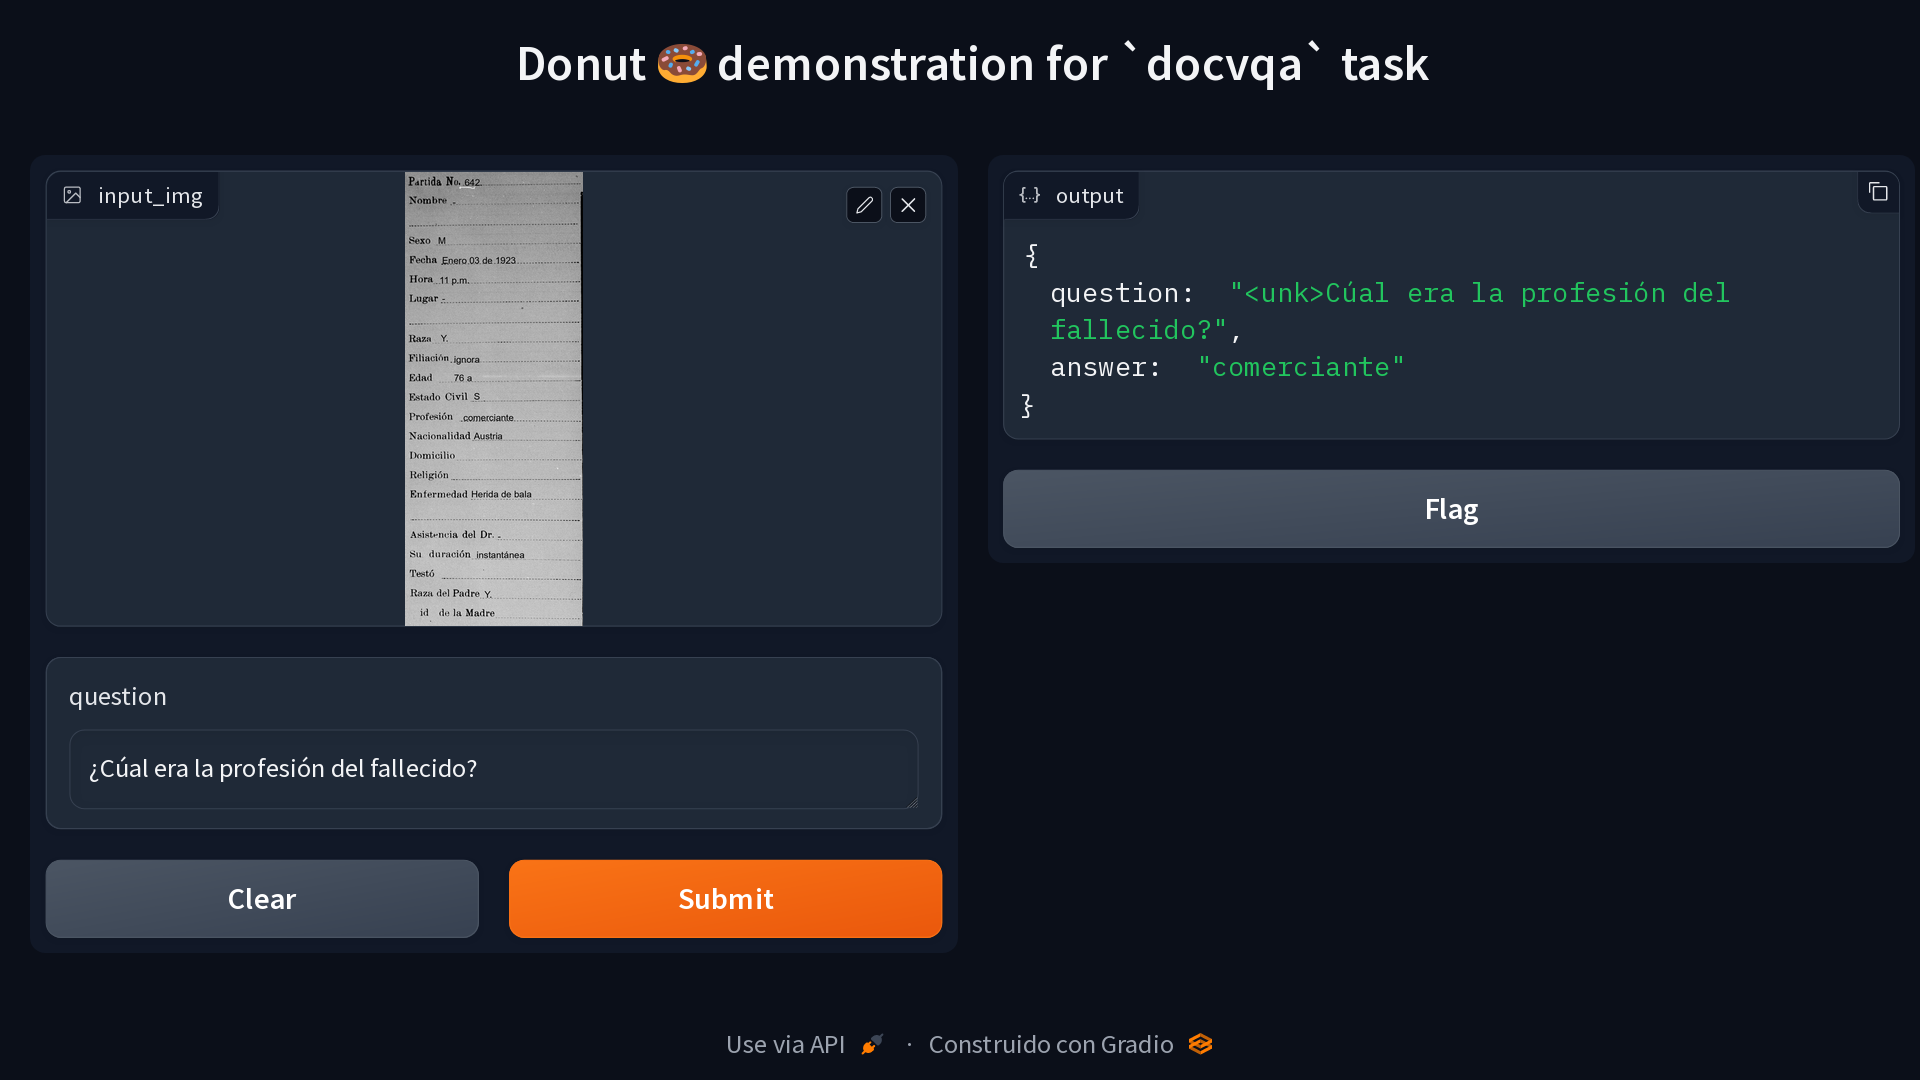
\includegraphics[width=0.9\textwidth]{docvqa.png}
	\caption{Ejemplo de inferencia}
	%\label{fig:}
\end{figure}

%Esta sección reporta datos o información obtenida al aplicar la metodología propuesta sobre el problema encontrado. Estos deben cubrir tanto el objetivo general, como los objetivos (general y específicos). Los resultados de esta sección deben estar alineados con los resultados esperados planteados en la sub-sección Objetivos. Dependiendo del área donde pertenece la tesis, esta sección debe contener un Protocolo Experimental, o la construcción de modelos (UML por ejemplo), entre otros.

%Esta es la parte mas extensa, y debe cubrir completamente con lo que se desea demostrar o solucionar. No dude en utilizar esquemas, gráficos, etc, a fin de mostrar todo el trabajo realizado. Esta sección debería terminar con una discusión.

\section{Discusión}

Por problemas con el cluster Khipu, nos hemos visto limitados en el tiempo y tamaño del entrenamiento.
El modelo funciona, pero debido a la falta de data augmentation tiene problemas con documentos diferentes
a su dataset de entrenamiento.

%Finalmente, la presentación de los resultados suele ir seguida de la sección Discusión, aunque la división entre estas dos secciones no es rígida y pueden aparecer juntas como una parte estructural de un documento académico.

\end{document}
